\documentclass[times, 10pt]{thesisMDH}
\usepackage[ddmmyyyy]{datetime}
\usepackage[pdfborder={0 0 0},colorlinks=true,urlcolor=blue,citecolor=red,bookmarks=false]{hyperref}
\addbibresource{references.bib}

\fancyHeader{Short title of the thesis}{Authors}

\university{Mälardalen University}

\department{School of Innovation Design and Engineering\\ Västerås, Sweden}

\subject{Thesis for the Degree of Master of Science in Engineering - Robotics 30.0 credits}
\thesisTitle{Master Thesis Title}
\authorOne{Student Name1}{studentEmail@student.mdh.se}
\authorTwo{Student Name2}{studentEmail@student.mdh.se}

\examiner{Examiner\_Name}{Mälardalen University, Västerås, Sweden}
\supervisors{Supervisor\_Name}{Mälardalen University, Västerås, Sweden}
\companySupervisors{Supervisor\_Name}{Company name, location}

\theDate{\today} 

\begin{document}
\titlePage
% Begin actual text
\frontmatter
\section*{Introduktion: om begrepp som används i mallen}

I mallen använder vi ett antal begrepp som det är viktigt att ha klart för sig vad de avser och hur de relaterar till varandra.
Vi illustrerar detta med exempel.
Du kan ha fått ditt examensarbete som ett uppdrag från t ex ett företag.
I så fall har du ofta fått ett problem som företaget upplever och som du ska försöka hitta lösning på. 
Problemet utgör i detta fall bakgrunden till syftet med arbetet och den frågeställning som du arbetar fram.

Exempel: Företaget X har ett system som de vill kunna använda i en realtidstillämpning, men prestanda i systemet är okänt. 
Problemet är då: Prestanda i systemet är okänt.
Lösningen på problemet är att mäta prestanda.
Syftet med ditt arbete blir att kartlägga systemets prestanda så att du får ett mått på detta. 
Frågeställningen kan formuleras som: Vad är systemets prestanda? Motivationen för arbetet är att det är viktigt att känna prestanda när systemet ska användas för realtidstillämpningar.
När du har syfte och frågeställning klar formulerar du de mål som du ska uppfylla med arbetet, i det här fallet kan målen t ex vara att mäta ett antal olika aspekter av prestanda. 
Tillsammans kommer dessa mål då att uppfylla syftet. 
Men ditt examensarbete behöver inte vara formulerat som ett specifikt problem som ska lösas.
Andra exempel på arbeten som kan förekomma som examensarbeten kan vara:
\begin{itemize}
\item[--]	``Case study'' eller studie av något fenomen
\item[--]	Litteraturstudie
\item[--]	Undersöka något, t ex hur användare interagerar med en mjukvara eller hur en design kan anpassas till en viss grupp användare
\item[--]	Analysera t ex jämföra prestanda hos olika programvaror
\item[--]	Utvärdera hänger ofta ihop med att analysera något, din uppgift kan vara att lämna en rekommendation om vilket verktyg som bäst lämpar sig för en viss uppgift
\item[--]	Utforska ny teknik eller nya angreppssätt. I detta kan ingå att utveckla en artefakt, t ex en mjukvara eller ett system. 
\item[--]	Utreda en frågeställning, t ex genom att göra en förstudie
\item[--]	Utveckla och utvärdera en algoritm, t ex för ett beräkningsproblem
\end{itemize}
Naturligtvis kan ditt examensarbete också innehålla flera av ovanstående komponenter. 
Gemensamt för alla examensarbeten är att de ska vara grundligt vetenskapligt förankrade, ett examensarbete får t ex inte vara enbart en implementation.

I många av exemplen ovan finns det inte något tydligt specificerat problem som ska lösas. 
Det kan istället röra sig om en fråga som du söker svar på, som i exemplet med utvärdering.
Men alla examensarbeten ska ha syfte, frågeställning och motivation. 
Frågeställningen ska vara utformad så att den går att besvara på något sätt genom det arbete du gör.
Men svaret kan vara abstrakt, det kan t ex vara att bidra till kunskap om frågeställningen.
I exemplet där uppgiften är att utforska en teknik, så skulle frågeställningen kunna vara ”Vilka problem finns med att utveckla XX”?
Det är också vanligt att arbetet innebär att du ska analysera och/eller utvärdera artefakten du utvecklat.
Frågeställning och syfte ska matcha varandra på så sätt att när syftet är uppnått så besvaras frågeställningen.
I texten kommer vi att använda begreppet uppgift för det du ska göra, vare sig det är ett problem som ska lösas eller något annat.
Texten i mallen är i denna version på svenska, men för varje rubrik finns motsvarande engelska ord inom parentes.

Denna sida ska inte ingå i slutrapporten
\newpage % Remove 000-guideline section
% ============================= Abstract ==============================
\begin{abstract}
Det här avsnittet ska helt enkelt vara just detta: en sammanfattning av hela rapporten. En lämplig omfattning är c:a 200 – 250 ord.  En bra tumregel är att sammanfattningen ska hållas så kort det går, den ska vara kompakt men fortfarande tydlig, informativ och väcka intresse. Ge de viktigaste fakta
och summera allt det som är väsentligt i rapporten.  Följande bör ingå:
\begin{itemize}
\item[--]	Presentation/introduktion av området för arbetet
\item[--]	översiktlig presentation av uppgiften inklusive syfte och frågeställning
\item[--]	Motivation till varför området och uppgiften är viktiga och intressanta
\item[--]	Generell beskrivning av hur du angripit uppgiften, vad du har gjort
\item[--]	Sammanfattning av resultat och slutsatser och vad ditt arbete bidrar med
\end{itemize}

Inga detaljer ska vara med i sammanfattningen, inte heller beskrivning av hur rapporten är uppställd. 
Sammanfattningen ska kunna läsas helt fristående från resten av rapporten, och av en ganska bred grupp av läsare. Den ska ge en bra grund för att en läsare ska kunna bedöma om hen är intresserad av att läsa hela rapporten. 
Sammanfattningen är den del av en rapport som läses allra mest och av flest personer. Därför är det extra viktigt att du skriver en bra sammanfattning. Du behöver ha ett ordentligt grepp om innehållet i rapporten när du skriver sammanfattningen, och när hela rapporten är klar bör du granska och vid behov revidera sammanfattningen så att den överensstämmer med rapporten.

\end{abstract}
\newpage
%========= Tables ==========
{\hypersetup{linkcolor=black}\tableofcontents}
\clearpage
{\hypersetup{linkcolor=black}\listoffigures}
\clearpage
{\hypersetup{linkcolor=black}\listoftables}
 
\mainmatter
% ===== Content: Modify the structure according to your needs =======
\section{Introduction}
\label{sec:intro}
Le présent rapport expose les travaux réalisés dans le cadre du cours Deep Learning II du Master Data Sciences de l'Institut Polytechnique de Paris. \\
L'étude porte sur la comparaison des performances en termes de précision de deux types de réseaux neuronaux: l'un pré-entraîné, l'autre initialisé de manière aléatoire. Les tests ont été effectués en modifiant différents paramètres, tels que le nombre de données d'apprentissage, le nombre de couches du réseau et le nombre de neurones par couche. 
Le but de l'étude était de classifier des images de chiffres manuscrits issus de la célèbre base de données MNIST.

\section{Étude sur Binary AlphaDigit}
Afin de vérifier la pertinence et la cohérence de nos programmes train\_RBM et train\_DBN que nous avons implémenté précédemment, nous allons nous concentrer sur l'étude exclusive de la base de données Binary AlphaDigit. Cette approche nous permettra de tester et de valider nos fonctions et notre approche. 

\subsection{Réseau Restricted Boltzmann Machines (RBM)}
Nous avons initié une série de tests non supervisés en utilisant un RBM avec les paramètres suivants:
\begin{itemize}
    \item Itération : 200
    \item Taux d'apprentissage : 0.1
    \item Taille des mini-batch : 32
\end{itemize}

Le modèle a été entraîné sur des données d'apprentissage appartenant à la classe du caractère '5', '6', 'H' et 'A'. Après entraînement du réseau RBM, la génération des images nous a donné le résultat suivant: 
\begin{figure}[H]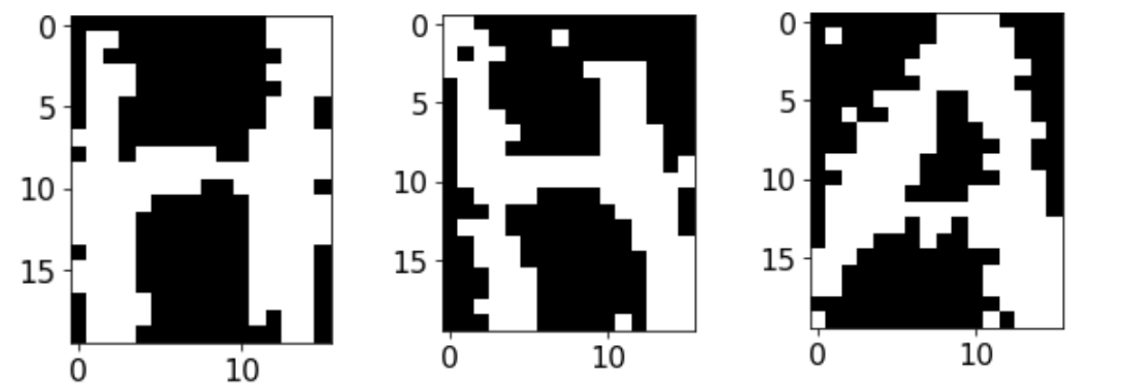
\includegraphics[width=140mm]{images/RBM.png}
\caption{génération de 3 images à l'aide du réseau RBM entraîné avec 4 chiffres}
\end{figure}

Il est évident que les images générées en sortie présentent une forte ressemblance avec les images d'entrée, tout en étant facilement identifiables et lisibles.

\subsection{Réseau Deep Belief Network (DBN)}
Nous allons reprendre les mêmes paramètres qui ont été utilisés pour l'entraînement du réseau RBM, que nous rappelons ci-dessous :
\begin{itemize}
    \item Itération : 200
    \item Taux d'apprentissage : 0.1
    \item Taille des mini-batch : 32
\end{itemize}
 
On obtient pour le DBN avec 3 couches et
200 neurones par couche:

\begin{figure}[H]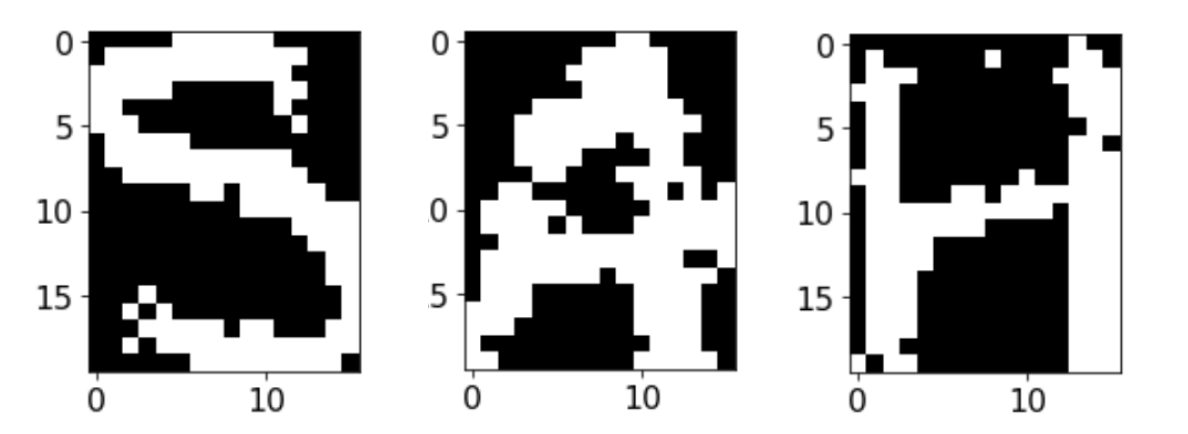
\includegraphics[width=140mm]{images/DBN.png}
\caption{génération de 3 images à l'aide du réseau DBN entraîné avec 4 chiffres}
\end{figure}

De manière générale, il est possible de constater que le DBN produit des images nettement plus lisibles que celles générées par le RBM.

En effet, les modèles génératifs tels que les RBM et DBN peuvent être limités en termes de la capacité à apprendre de nouveaux caractères, car ils nécessitent une grande quantité de données d'apprentissage pour capturer les variations subtiles entre les caractères. De plus, la complexité des modèles peut augmenter considérablement avec le nombre de caractères à apprendre, ce qui peut rendre l'apprentissage très lent et nécessiter des ressources informatiques importantes.
     

\newpage
\section{Etude sur MNIST}
\subsection{Comparaison de deux réseaux en fonction du pré-apprentissage} 

Dans cette section, nous allons évaluer les performances du Deep Neural Network sur le jeu de données MNIST en fonction de l'entraînement préalable du réseau. Nous allons examiner les performances pour différentes valeurs de paramètres, tels que le nombre de couches du réseau, le nombre de neurones par couche et la quantité de données d'entraînement utilisées. Pour toutes les comparaisons, nous avons utilisé un nombre fixe d'itérations pour les descentes de gradient, à savoir 100 pour les RBM et 200 pour l'algorithme de rétropropagation du gradient. De plus, nous avons utilisé un taux d'apprentissage de 0,1 et une taille de mini-batch de 64.


\subsection{Comparaison selon le nombre de couches}

\begin{figure}[H]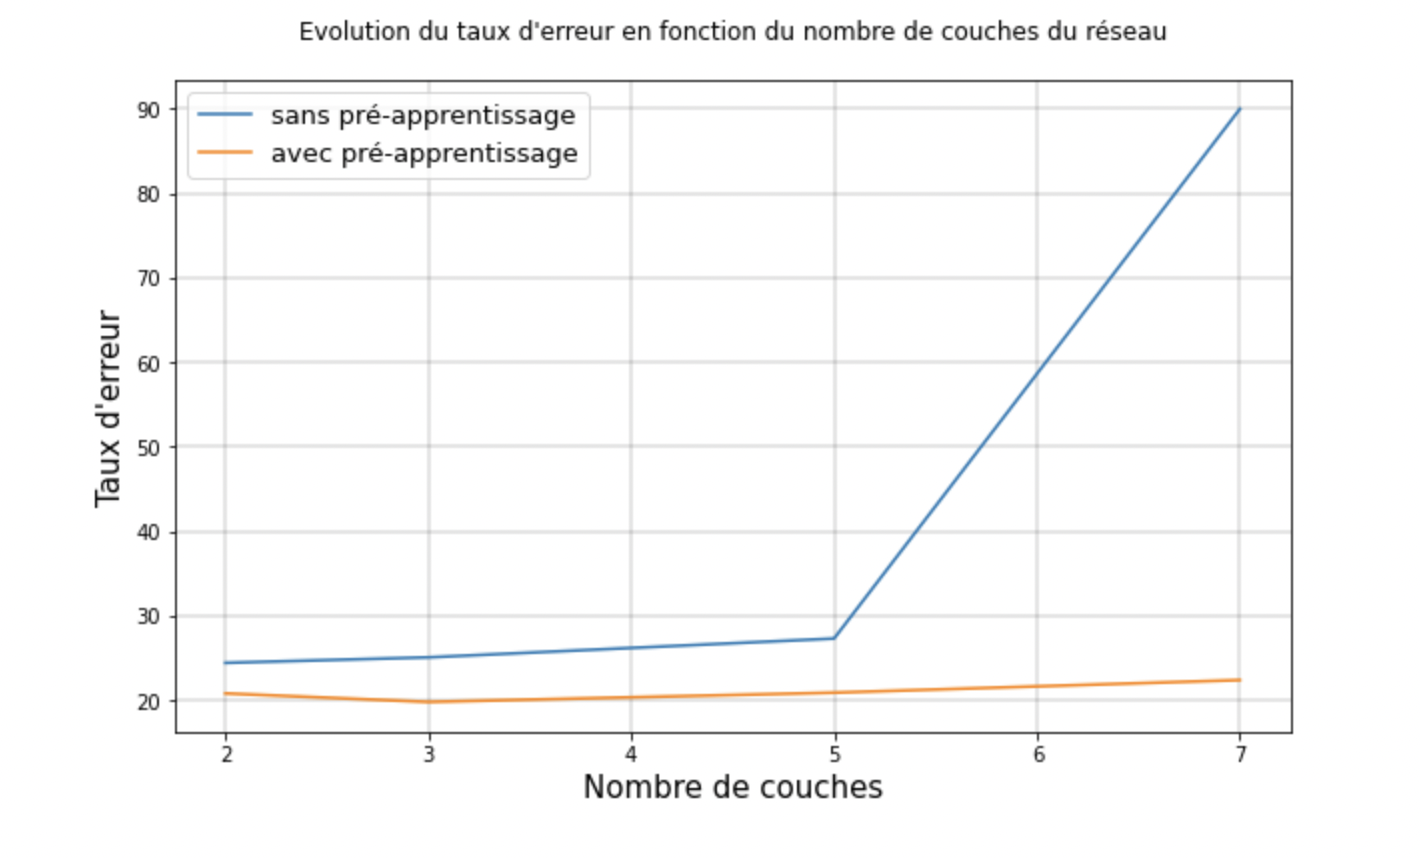
\includegraphics[width=140mm]{images/DNN1.png}
\caption{Variation du taux d'erreur en fonction du nombre de couches dans un DNN}
\end{figure}
En examinant la Figure 3, on constate que le nombre de couches n'a pas un impact significatif sur la précision, comme le montre le taux d'erreur (1-précision). Cependant, pour les réseaux sans entraînement préalable, on observe une forte augmentation du taux d'erreur à partir de 5 couches. Ces résultats ont été obtenus en utilisant 60000 données et un nombre de neurones par couche de 200.


\subsection{Comparaison selon le nombre de neurones par couches}

\begin{figure}[H]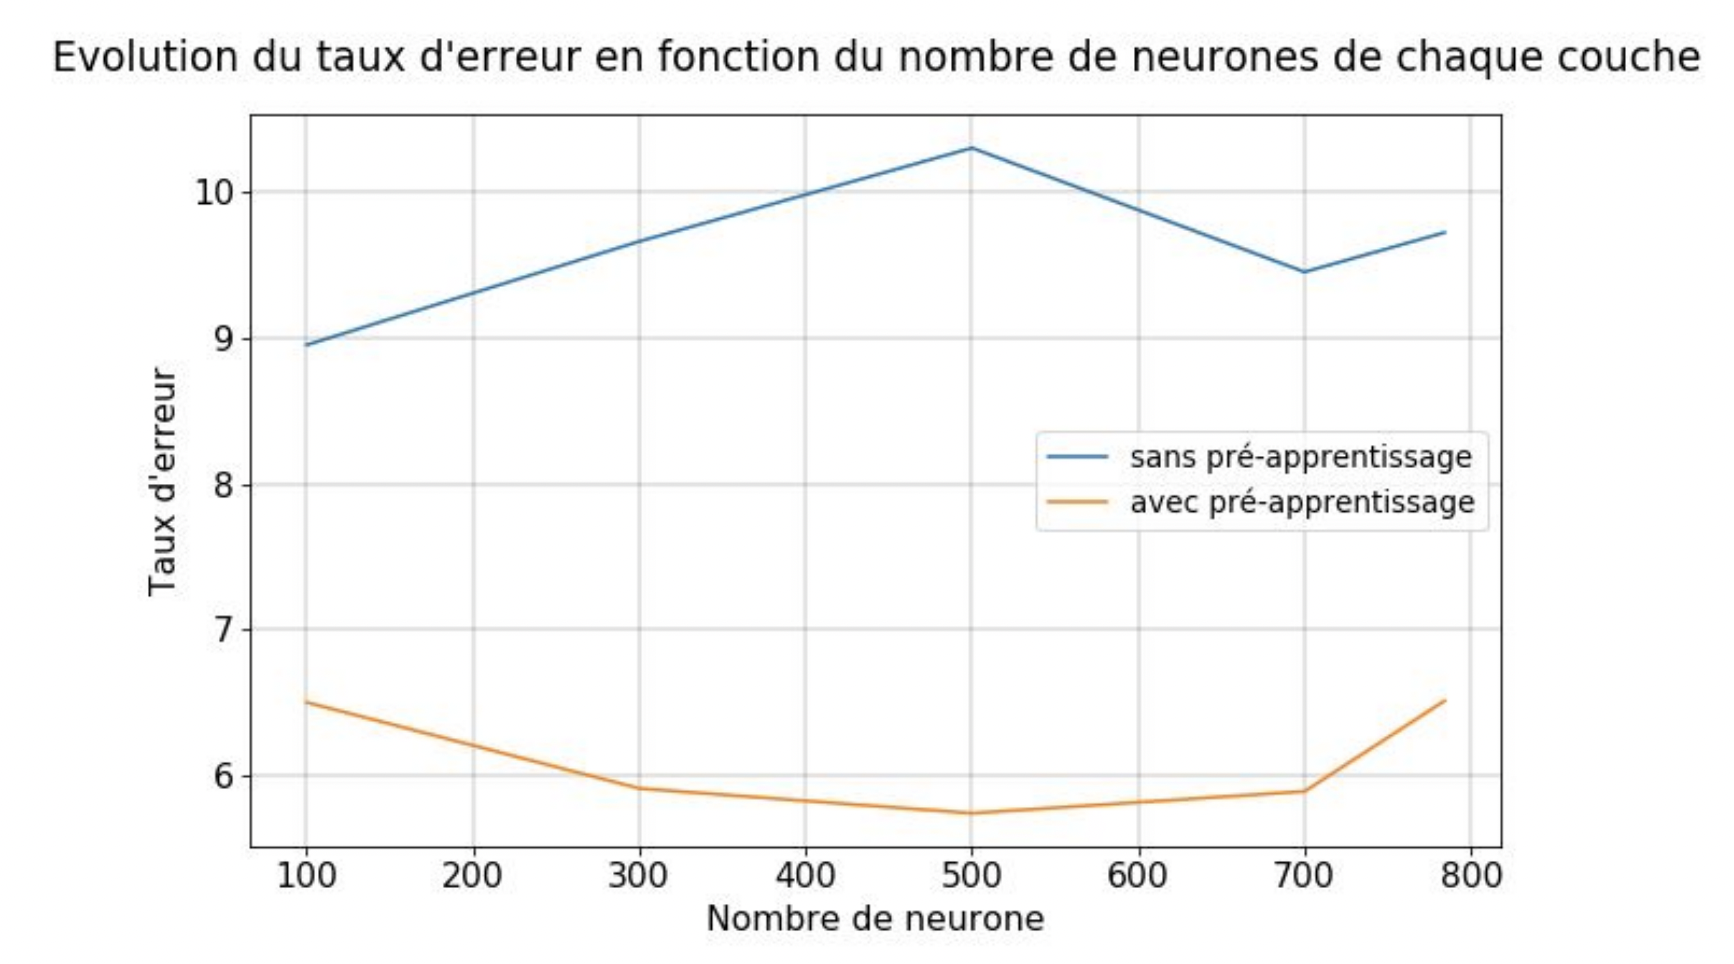
\includegraphics[width=140mm]
{images/graph1.png}
\caption{Taux d'erreur en fonction du nombre de neurones par couche}
\end{figure}
La Figure 4 révèle que la précision du réseau pré-entraîné augmente à mesure que le nombre de neurones par couche augmente. Cependant, pour le réseau non-entraîné, on observe une augmentation de l'erreur lorsque le nombre de neurones par couche est augmenté. Ces tests ont été réalisés en utilisant 2 couches et 60000 données.

\subsection{Comparaison selon le nombre de neurones par couches}

\begin{figure}[H]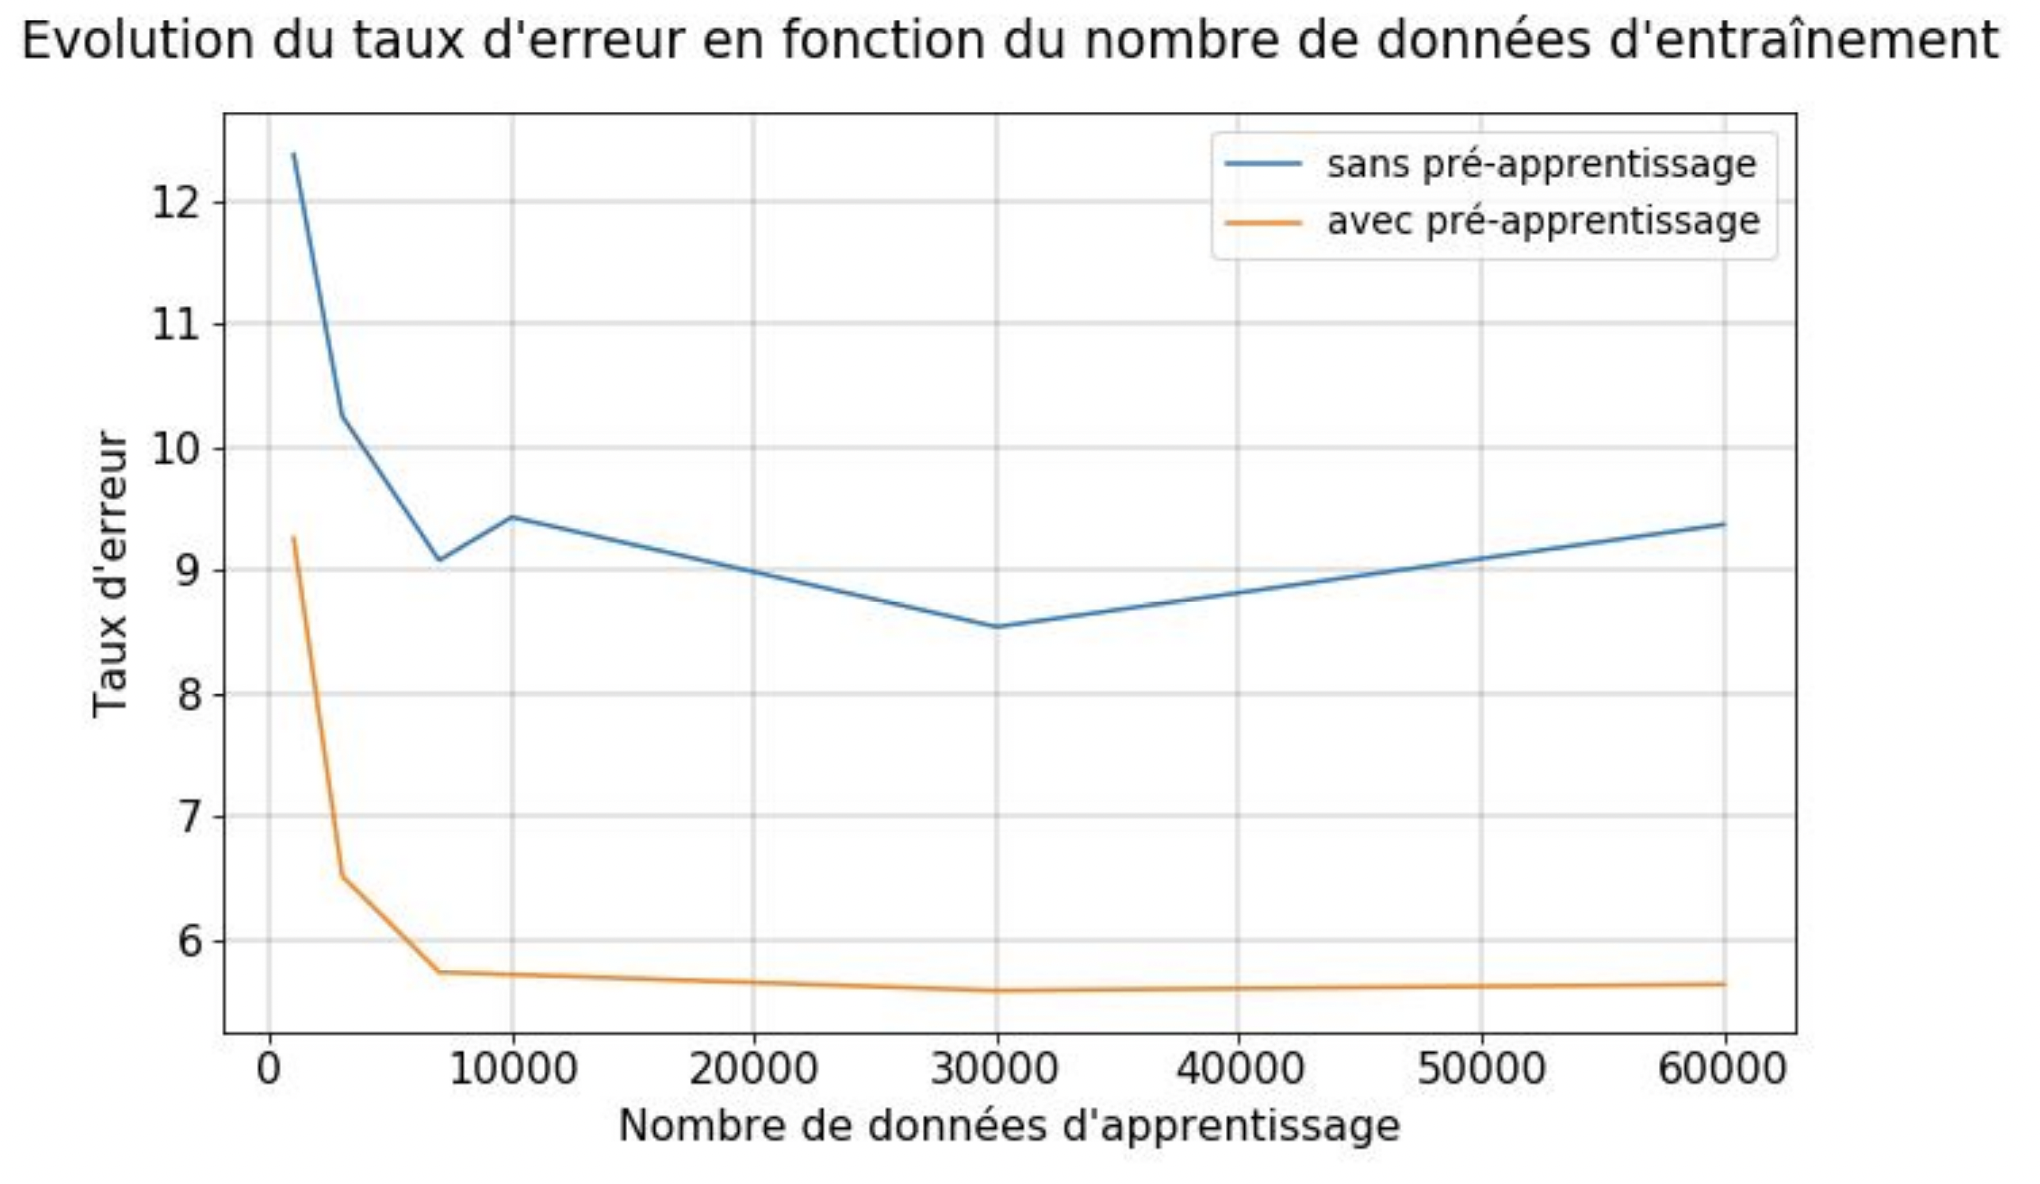
\includegraphics[width=140mm]
{images/graph2.png}
\caption{Variation du taux d'erreur en fonction de la quantité de données pour des DNN entraînés avec ou sans pré-apprentissage.}
\end{figure}
La Figure 5 indique que pour les deux réseaux, la précision augmente et l'erreur diminue à mesure que le nombre de données d'entraînement augmente. Cependant, on remarque également un taux d'erreur minimum lorsqu'on entraîne le réseau avec 30 000 données. Ces tests ont été réalisés en utilisant 2 couches et 200 neurones par couche.\\
En analysant ces trois comparaisons, on constate que le réseau pré-entraîné présente un taux d'erreur nettement inférieur à celui du réseau non-entraîné. Cependant, il convient de noter que le temps de calcul requis pour le pré-apprentissage est très élevé.

\subsection{Comparaison selon le learning rate}

La Figure 6 permet de déterminer le learning rate optimal pour un réseau entraîné avec 60 000 données, qui est de 0,425 dans notre cas. De manière générale, plus le LR est élevé, plus le taux d'erreur est bas. Cependant, la valeur de 0,425 permet une nette amélioration du taux d'erreur pour notre problème.

\begin{figure}[H]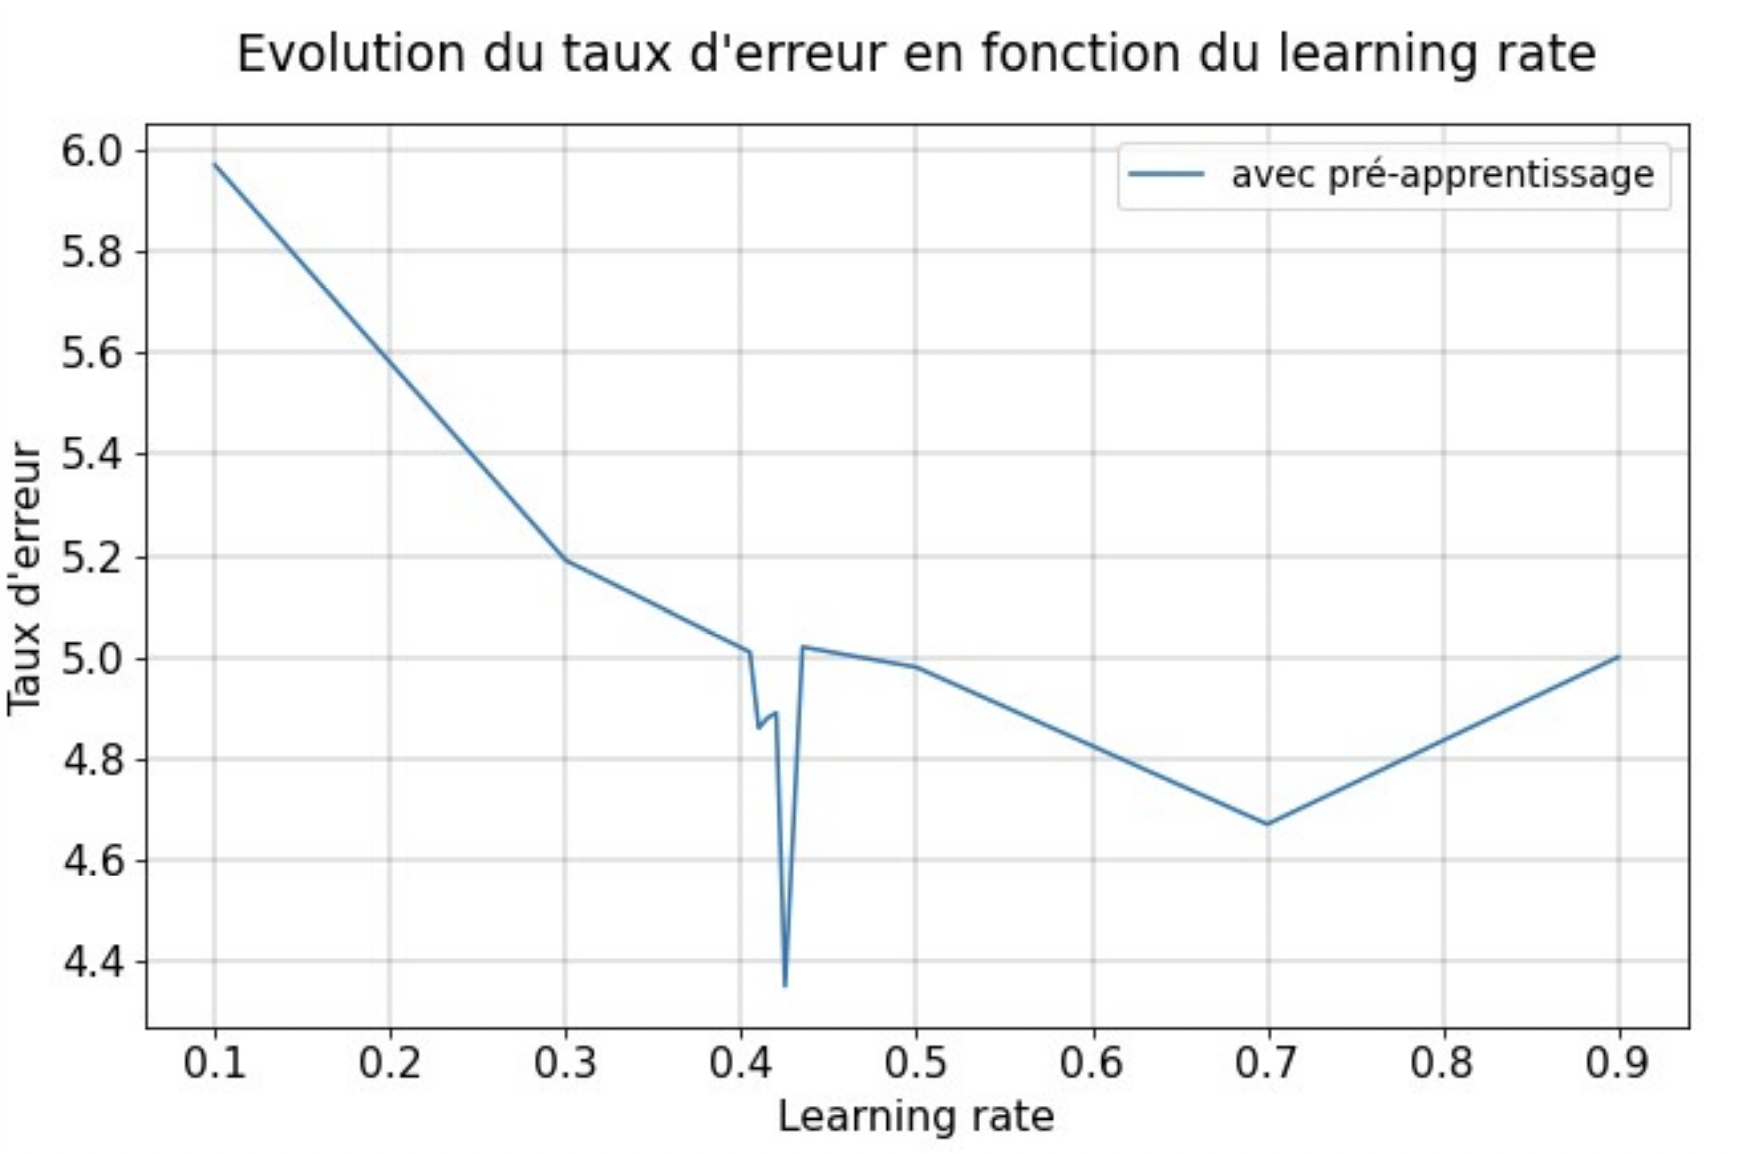
\includegraphics[width=140mm]
{images/graph3.png}
\caption{Variation du taux d'erreur en fonction du learning rate.}
\end{figure}

\subsection{Meilleur taux de classification}
En se basant sur les comparaisons précédentes, nous avons cherché à déterminer les paramètres optimaux pour obtenir le taux d'erreur le plus faible possible sur les données de test. Nous avons ainsi obtenu un taux d'erreur de 2,74\% en utilisant les paramètres présentés dans le tableau ci-dessous :


\begin{table}[h!]
\centering
\begin{tabular}{|c|c|}
\hline
Paramètre & Valeur \\
\hline
Nombre d’itérations (RBM)  & 100 \\
Nombre d’itérations (Rétro-Propagation) & 350  \\
Taille des mini-batch & 128 \\
Learning Rate & 0.425  \\
Nombre de données d’apprentissage & 30 000  \\
Nombre de couches & 4  \\
Nombre de neurones par couche & 200  \\
\hline
\end{tabular}
\end{table}
 %SOTA
\newpage
\section{Tidigare arbeten/litteraturöversikt (Related Work)}

Syftet med detta avsnitt är att placera in ditt arbete i ett sammanhang och jämföra det med tidigare publicerade arbeten och resultat inom området. Denna del ska vara grundlig. Du beskriver här existerande kunskap och hur denna utökas av ditt arbete. Den ska innehålla analyser av tidigare arbeten som exempelvis beskriver hur olika metoder skiljer sig åt. Du ska visa på de viktigaste likheterna och skillnaderna beträffande uppgift, angreppssätt/metodologi samt resultat. Det är viktigt att du på ett neutralt sätt diskuterar för- och nackdelar med ditt eget arbete jämfört med andras.

Detta skapar också en förväntan på bidraget för ditt arbete, läsaren lär sig här om begränsningar hos tidigare arbeten och varför din uppgift är en utmaning.. 

Tillsammans kommer detta avsnitt tillsammans med bakgrund att introducera ”state of the art”/”state of practice” och dess brister, betydelsen av uppgiften samt vad ditt arbete ska jämföras med.

\newpage
\section{Metod (Method)} 
\label{sec:method}

I det här avsnittet ska du beskriva vilka vetenskapliga metoder du har använt och hur du har gått tillväga med själva arbetet. För varje mål ovan identifierar du en metod för att nå målet. Valen av metod ska motiveras. Du kan t ex ha gjort en matematisk modell, använt simuleringar, gjort en implementation som du testat eller gjort experiment som du kanske utvärderat med hjälp av statistiska metoder. Vi avser här i första hand att du beskriver de vetenskapliga metoder du använt, men det är också bra om du ger en beskrivning av hur du arbetat med uppgiften. Avsnittet Metod svarar också på varför du gjorde på ett visst sätt eller varför du använde ett visst verktyg. Du ska alltså inte bara beskriva ”vad” utan  också ”varför”. Ställ dig frågan: kan den valda metoden hjälpa mig att nå de uppsatta målen och därmed besvara frågeställningen?

Att välja rätt vetenskapliga metod(er) är viktigt för att du ska nå dina mål, därför är detta en punkt som du på ett tidigt stadium bör diskutera med din handledare. Sök också i litteraturen efter bra beskrivningar av metoder, och hur du på bästa sätt skriver ett Metodavsnitt. 

\newpage
\section{Etik och Samhälleliga aspekter (Ethical and Societal Considerations)}

I först hand avser vi med ”etik” här forskningsetiska frågor. Innebär ditt val av frågeställning eller metod något forskningsetiskt ställningstagande? Om du till exempel intervjuar personer för ditt arbete, kan du garantera dessa anonymitet och på vilket sätt använder du den information du får av dem? Finns det andra etiska aspekter att beakta i arbetet? Kan det finnas etiska aspekter på resultatet av ditt arbete? Du bör tydligt ange om du anser att ditt arbete inte innehåller några forskningsetiska frågor. 

Du ska också kritiskt granska och analysera ditt arbete med hänsyn till samhälleliga aspekter. Här kan du till exempel diskutera hur ditt arbete förhåller sig till mål som ekonomisk, social och ekologiskt hållbar utveckling. Det kan också finnas juridiska och politiska aspekter på ditt arbete. 

\newpage
\section{``Beskrivning av arbetet''/ ``Description of the work'') }

Efter avsnitten ovan följer nu en beskrivning av vad du gjort. Du ska inte använda rubriken ovan, utan ersätta den med lämpliga rubriker, beroende på ditt arbete. Strukturen ska göras tydlig genom avsnittsrubrikerna. Det är viktigt med en klar och tydlig logisk struktur och ett berättande flöde. Du ska ha med avancerad bakgrundskunskap som är nödvändig för att förstå hur du löst uppgiften, och definiera hypoteser och viktiga begrepp. Beskrivning av experiment ska vara sådan att det ska gå att upprepa experimenten. Om en sådan beskrivning blir väldigt lång och detaljerad kan du lägga den i en bilaga, se nedan.  



\newpage
\section{Resultat (Results)}

Här kan du till exempel presentera resultat av experiment, bevis, analys av data etc. Dina resultat måste beskrivas så tydligt att en läsare kan bedöma dem.  Du ska också förklara och analysera resultaten.



\newpage
\section{Diskussion (Discussion)}

Här presenterar du tolkning av resultaten och bedömer deras signifikans. Diskutera möjliga konsekvenser av resultaten, och presentera eventuella rekommendationer. Det är viktigt att du redogör för om du uppnått de mål du satte upp och därmed besvarat din frågeställning och uppnått syftet med arbetet. Avsnittet ska också innehålla reflektioner kring arbetet, som till exempel dess begränsningar.  Du kan också diskutera lösningar på problem som du identifierat och diskuterat tidigare, eller ta upp andra problem som arbetet inte behandlat, frågor som ej besvarats. Koppla också dina resultat till tidigare arbeten. På så sätt kan diskussionen bli ett samtal med det du skrev i tidigare avsnitt.  Slutligen ska du sätta ditt eget arbete i ett större sammanhang, bredda ditt perspektiv. Kan dina resultatet generaliseras? Kan det du gjort användas i något annat sammanhang? 

\newpage
\section{Slutsatser (Conclusions)}

I detta avsnitt ska du summera rapporten samt presentera slutsatser och slutanalys. Ge en kort översikt av syftet och frågeställningen. Du ska sedan tydligt tala om de viktigaste resultaten, förklara deras signifikans och sätta in dem i sitt sammanhang. Alla slutsatser ska ha stöd i tidigare delar av rapporten.  Du ska däremot inte presentera nya detaljer. 

En expert ska kunna läsa detta avsnitt oberoende av resten av rapporten. 


\newpage
%\input{sections/Acknowledgments}
% ============================= References ============================
% \newpage
\printbibliography
\addcontentsline{toc}{section}{References}
\printbibliography
\addcontentsline{toc}{section}{name}

% ============================ Appendices =============================
%\newpage
%\begin{appendices}

	%\input{appendices/appendices1}
	%\clearpage
	
	%\input{appendices/appendices2}
	%\clearpage
	
%\end{appendices}

\end{document}
